\documentclass[a4paper,10pt]{article}

\usepackage{fancyhdr}
\usepackage{graphicx}
\usepackage{geometry}
\geometry{a4paper, left=2cm, right=2cm, top=1.5cm, bottom=3cm }
\usepackage{caption}
\usepackage{subcaption}
\usepackage{hyperref}
\usepackage{natbib}

\usepackage{etoolbox,fancyhdr,xcolor}
\newcommand{\headrulecolor}[1]{\patchcmd{\headrule}{\hrule}{\color{#1}\hrule}{}{}}
\newcommand{\footrulecolor}[1]{\patchcmd{\footrule}{\hrule}{\color{#1}\hrule}{}{}}
\renewcommand{\headrulewidth}{1pt}
\headrulecolor{red!100}%
\renewcommand{\footrulewidth}{1pt}
\footrulecolor{red!100}%

\fancyhf{}
\fancyhead[R]{
\includegraphics[width=0.25\textwidth]{UoBLogo.png}}

\fancyfoot[L]{CS 725 Project Interim Report}
\fancyfoot[C]{IIT Bombay}
\fancyfoot[R]{\thepage}

\setlength{\headheight}{15mm}
\pagestyle{fancy}

\bibliographystyle{apalike}

\usepackage{times}
\begin{document}

\noindent 
\begin{center}
\textbf{{\large Interim Report \\ \Large Ground Motion Prediction using Neural Network}} \\
\end{center}


\noindent 
\textbf{Authors:}

\hspace{1 cm} Anis M.V. (23D0292) \\

\hspace{1 cm} Moh. Zaid (22D1264) \\

\hspace{1 cm} Ashwin (23M2153) \\

\hspace{1 cm} Vishnu T.S. (22N0413) \\

\noindent 
\textbf{Project GitHub Page (Under development):}

\hspace{1 cm} \href{https://github.com/anismhd/CS725_Project}{GitHub} ($https://github.com/anismhd/CS725_Project$) \\


\section{Abstract}

Historically, seismic events have brought extensive destruction and distress to communities worldwide.
These events have potential to generate economic losses of up to a staggering \$200 billion (Japan, 1995).
In the current year alone, over 50,000 lives were tragically lost due to earthquakes(Turkey Earthquake).
The most devastating consequence of earthquakes is the ground vibration, which can inflict damage to infrastructure causing huge economic losses.
Throughout history, the prediction of this ground motion has remained a challenge for seismology groups. 
Researchers have explored various empirical equations, commonly known as attenuation equations or Ground Motion Prediction Equations (GMPEs), to estimate ground motion to engineer communities towards more seismic resilience. 
These empirical relationships were always challenged by new events or information. 
Recent studies in this field have explored the use of neural networks for the prediction of ground motions. 
In this project, we intent on an exploration of the application of neural networks in predicting ground motions, aiming to assess their effectiveness in comparison to traditional empirical equations.

\section{Brief Overview on Ground Motion Studies}
The Earth's crust is comprised of tectonic plates that constantly move relative to one another.
This movement generates stress along the plate boundaries and faults.
When this stress exceeds a critical threshold, it triggers a sudden slip or movement at the boundary, releasing the accumulated energy in the form of waves.
The energy released propagates as waves across the plate boundary, causing ground vibrations. 
Seismographs are used to measure these vibrations, which scientists and engineers analyze to study and characterize future earthquakes and mitigate seismic vulnerabilities. 

Historically people has attempted to charcterise these ground motions/vibrations. 
The common parameters is peak ground accelartion (PGA), which is the highest ground accelaration measured at free ground.
Eventhough PGA provides intusion on ground shaking intensities, the behaviour of buildings/structures under ground motions are best described by Response Spectra.
It represents the maximum response of a structure to ground motion at various frequencies. 
In simpler terms, it shows how much a building or structure might shake at different levels of earthquake intensity, allowing engineers to design structures that can withstand these movements. 
By using this tool, they can create safer and more resilient buildings that can better withstand the forces of an earthquake. A typical process of estimating response spectra from ground motion is shown in Figure \ref{rsp}.

\begin{figure}[ht]
\centering
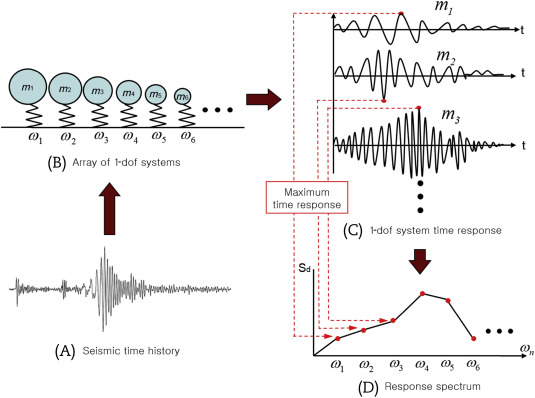
\includegraphics[height=6.6cm]{gm.jpg}
\caption{Pictorial representation of generation of response spectra}
\label{rsp}
\end{figure}

Historically people has attempted to prepare database of such ground motion parameters recorded across the world.
Various attempts were made by individually various institutions.
The PEER research group had prepared more transperent version of such database.
The present studies consider this database for development of ground motion prediction model.
A brief overview of the database and preliminary discussion on data collected are discussed in the following section.

\section{PEER Database of Ground Motion}
Tern of the century, PEER group initiated a large research program to develop Next Generation Attenuation equation, termed as project "NGA".
The project initially focused on development of common high-quality ground-motion database which can be accessed by all researchers around the globe.
Earthquake ground motion records from various recording stations around the globe were collected and processed using common procedure to enure coherency.
A total of 335 earthquake events with multiple station records were collected and stored at common point. Locations of these ground motion are shown in Figure \ref{NGA};

\begin{figure}[ht]
\centering
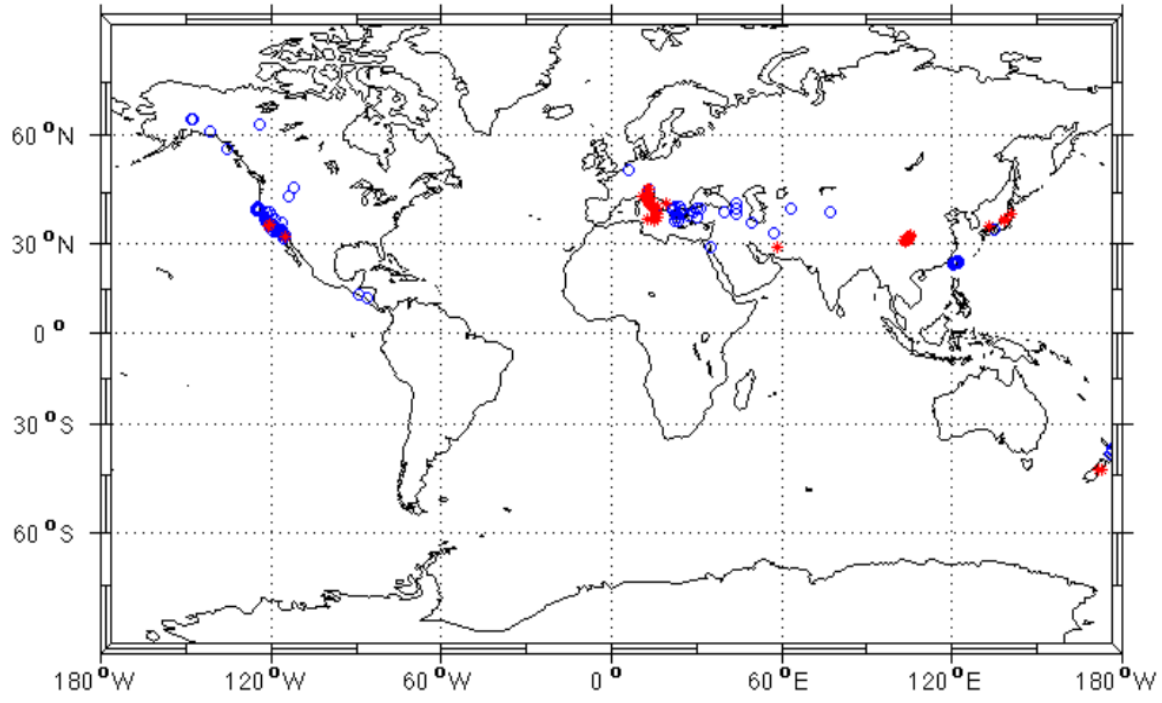
\includegraphics[height=6.6cm]{NGA_data}
\caption{List of Earthquakes Considered in the Study}
\label{NGA}
\end{figure}

\section{Ground Motion Prediction Models}
Variety of procedures were proposed for prediction of ground motion. 
The common procedure was empirical method, where functional form of ground motions are estimated through regression.
The functions forms is often expressed in terms of parameters characterizing the  earthquake source, travel-path and recording site.
The common parameters are;
\begin{enumerate}
	\item Magnitude of earthquake. This expresses quantity of energy released in log scale.
	\item Distance to source from site.
	\item Site Characteristics
\end{enumerate}

For the present study above parameters are considered.

\section{Development of Ground Motion Prediction Model (Implementation)}
Multilayer Perceptrons (MLP) are often used in regression applications. The MLP's are very effcient in nonlinear regressions. 
The general regression is estimation of conditional density model of the form


$$ p(y | x; \theta) = N(y | f_{\mu}(x;\theta), f_{\sigma}(x;\theta)^2) $$

Where;

$f_{\mu}(x;\theta)$ predicts the mean, and $f_{\sigma}(x;\theta)^2)$ predicts the variance.

In ground motion prediction equations, it is common to assume that the variance dependent of the input. 
This is called heteroskedastic regression.
The applications of Neural Network for the GMPEs, so far has been limited to homeostatic regression.
This study would attempt an novel approach to develop an model using Bayesian MLP, which capture mean and standard deviation of predictions correctly.
The advantage of the such model is the ability to estimate confidence interval of prediction, which are often critical in seismic mitigation studies and insurance studies.

\subsection{Heteroskedastic Regression}
The traditional MLP by default don’t report the uncertainty of their estimates.
The uncertainty in neural network computation can be considered through Bayesian neural network which often has two “heads”. One head will predict the value of the estimate, and the other to predict the uncertainty of that estimate. This dual-headed structure allows the model to dynamically adjust its uncertainty estimates, and because it’s a Bayesian network, also captures uncertainty as to what the network parameters should be, leading to more accurate uncertainty estimates.

The project aims to develop a ground motion prediction equation using two headed beyesian neural network. As part of the work following activities are carried out;

\subsection{Data collection and processing}

\begin{verbatim*}
implemented in following Jupyter Notebook files

1. Process Data.ipynb
2. Checking Processed Data
\end{verbatim*}

The PEER database is distributed in MS Excel file, which are read and converted to pandas DataFrame. The each feature of database are studied based on the manual shared by PEER Report (data/manual.pdf). The database had few records which were incomplete. These records were marked with placeholder "-999" character. These records were removed and datasets with complete information were selected for regression studies. The processed datasets were checked for its trend and variation with magnitude and distance. These plots are shown in Figure \ref{fig:datasets} and \ref{fig:datasets2}.


Based on the study of datasets, feature parameters that needs to considered in the regression model were identified.

\subsection{Prediction of Ground Motion using MLP}

Before venturing into Bayesian NN, the efficacy of NN to prediction ground motion were explored using MLPs. A comparison of observation and prediction are shown in Figure \ref{MLP}. It can be observed that the MLP models are capable of predicting functional form of ground motion prediction.

\begin{figure}[h]
\centering
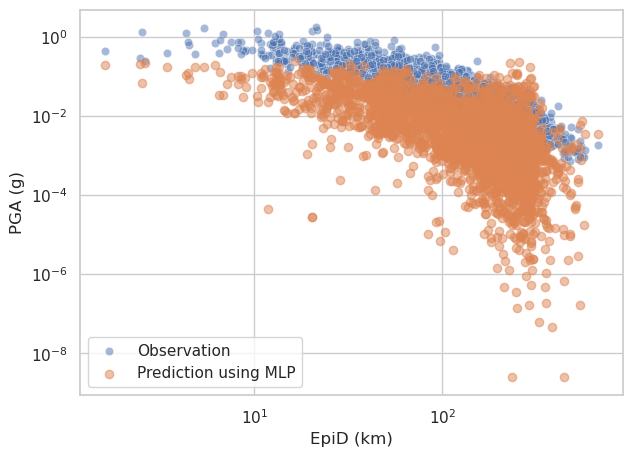
\includegraphics[height=8cm]{PGA_Pred}
\caption{Comparison of Results of MLP Model and Observation}
\label{MLP}
\end{figure}

\section{Summary of Activities Completed and Future Work}

\begin{enumerate}
	\item Data collection [\textbf{Completed}]
	\item Processing of Data [\textbf{Completed}]
	\item Development of ground motion prediction model using MLP [\textbf{Completed}]
	\item Development of Single Headed Bayesian Neural Network Model [\textbf{Progress}]
	\item Development of Two Head Bayesian Neural Network Model [\textbf{Pending}]
\end{enumerate}

\begin{figure}[h]
     \centering
     \begin{subfigure}[b]{0.45\textwidth}
         \centering
         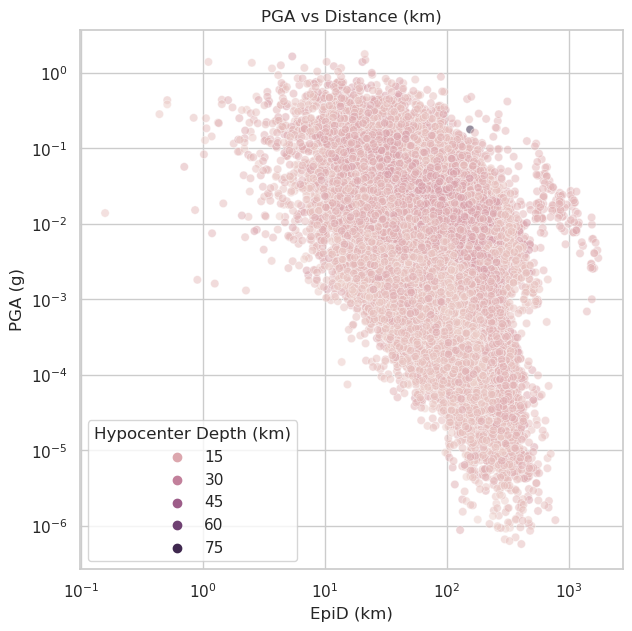
\includegraphics[width=\textwidth]{PGA_distance_Depth}
         \caption{Variation of PGA with Distance and Hypocenter Depth}
     \end{subfigure}
     \hfill
     \begin{subfigure}[b]{0.45\textwidth}
         \centering
         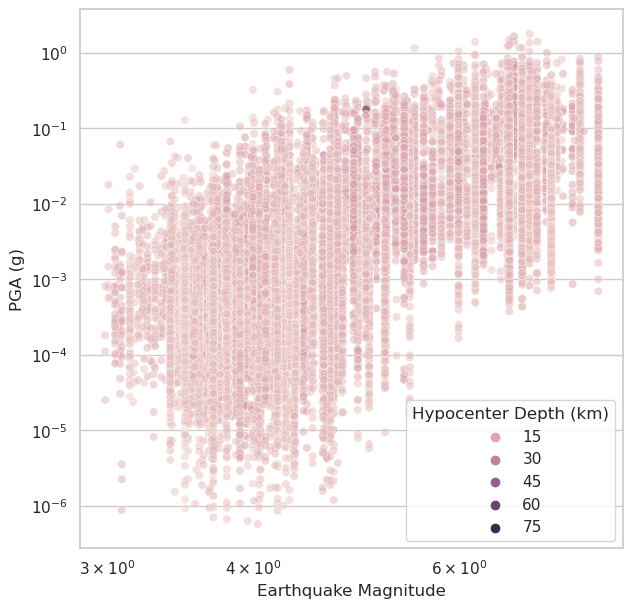
\includegraphics[width=\textwidth]{PGA_Mag_Depth}
         \caption{Variation of PGA with Magnitude and Hypocenter Depth}
     \end{subfigure} \\
     \begin{subfigure}[b]{0.45\textwidth}
         \centering
         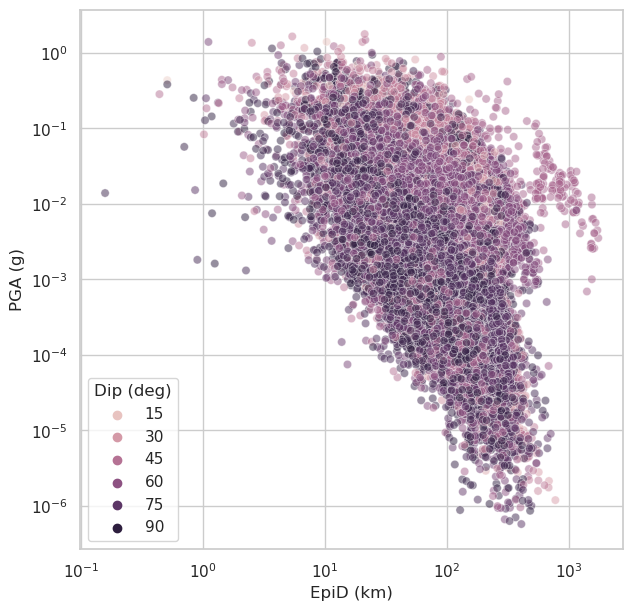
\includegraphics[width=\textwidth]{PGA_distance_Dip}
         \caption{Variation of PGA with Distance and Dip}
     \end{subfigure}
     \hfill
     \begin{subfigure}[b]{0.45\textwidth}
         \centering
         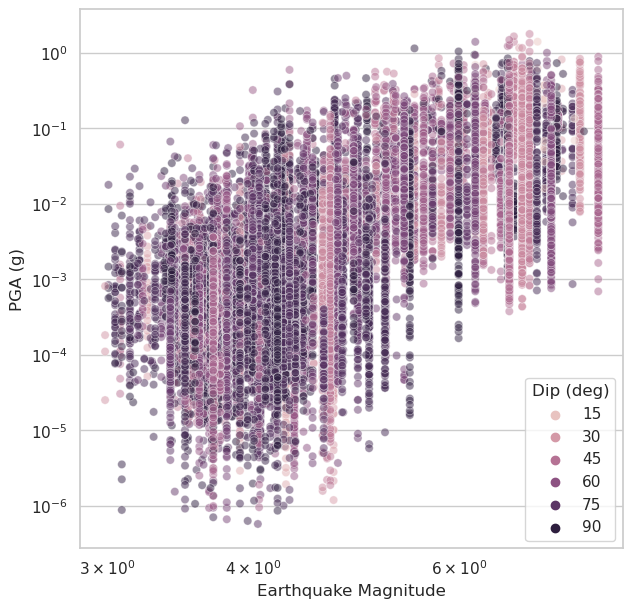
\includegraphics[width=\textwidth]{PGA_Mag_Dip}
         \caption{Variation of PGA with Magnitide and Dip}
     \end{subfigure} \\
     \caption{Study of Variation of PGA with Various Feature Parameters (1/2)}
        \label{fig:datasets}
\end{figure}

\begin{figure}[h]
     \centering
     \begin{subfigure}[b]{0.45\textwidth}
         \centering
         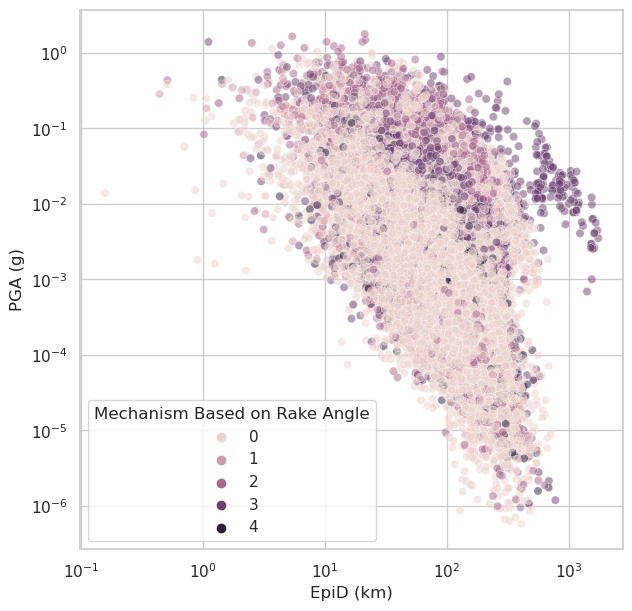
\includegraphics[width=\textwidth]{PGA_distance_Mechanism}
         \caption{Variation of PGA with Distance and Rake Angle}
     \end{subfigure}
     \hfill
     \begin{subfigure}[b]{0.45\textwidth}
         \centering
         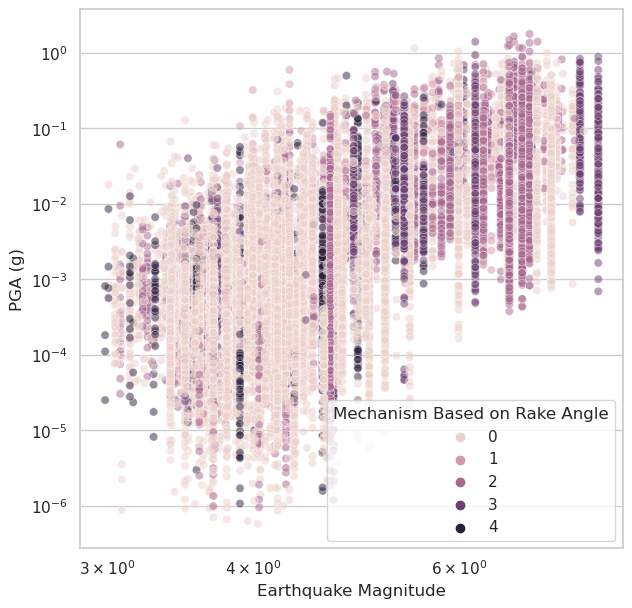
\includegraphics[width=\textwidth]{PGA_Mag_Mechanism}
         \caption{Variation of PGA with Magnitude and Rake Angle}
     \end{subfigure} \\
     \begin{subfigure}[b]{0.45\textwidth}
         \centering
         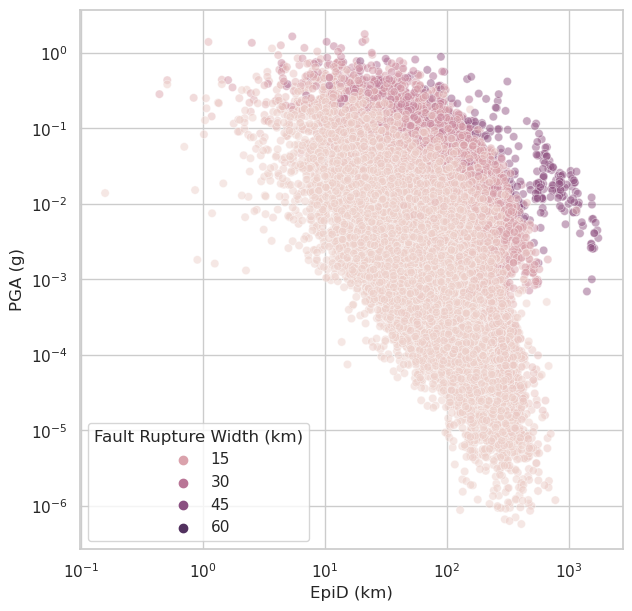
\includegraphics[width=\textwidth]{PGA_distance_Width}
         \caption{Variation of PGA with Distance and Width}
     \end{subfigure}
     \hfill
     \begin{subfigure}[b]{0.45\textwidth}
         \centering
         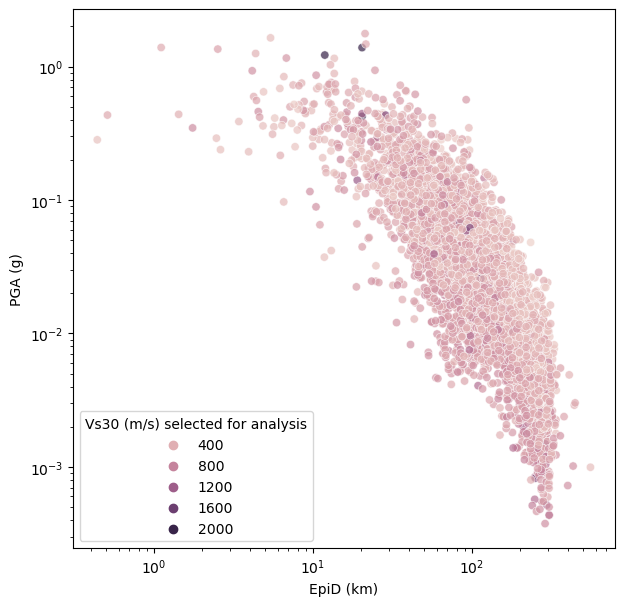
\includegraphics[width=\textwidth]{PGA_Mag_Width}
         \caption{Variation of PGA with Magnitude and Width}
     \end{subfigure} \\
        \caption{Study of Variation of PGA with Various Feature Parameters (2/2)}
        \label{fig:datasets2}
\end{figure}


\fontsize{8}{9}\selectfont
\bibliography{ResearchPaperBib}



\clearpage



\end{document}